%!TeX program = xelatex

% Define document font, paper size and type %
\documentclass[12pt,a4paper,numbers=noenddot]{scrreprt}

% Include all auxiliary packages
% All required packages to be used within this project

% Margin definitions
\usepackage[a5paper,vmargin=2cm,hmargin=1.5cm]{geometry}

% Packages to be used
\usepackage{fontspec}
\usepackage{eurosym}
\usepackage{amssymb}
\usepackage{mathtools}
\usepackage{amsmath}
\usepackage{upquote}
\usepackage{microtype}
\usepackage{longtable,booktabs}
\usepackage{graphicx}
\usepackage{grffile}
\usepackage{appendix}
\usepackage{float}
\usepackage{pst-all}
\usepackage{geometry}
\usepackage{xcolor}
\usepackage{xpatch}
\usepackage{nccmath}
\usepackage{subcaption}
\usepackage{xcolor}
\usepackage{multirow}
\captionsetup{compatibility=false}
\usepackage[crop=off]{auto-pst-pdf}
\usepackage[normalem]{ulem}

% Custom links color
\definecolor{linkscolor}{rgb}{0.89, 0.26, 0.2}

\usepackage[unicode=true,bookmarks=true,bookmarksopen=false,
  bookmarksopenlevel=1,pdfborder={0 0 0},backref=false,
  colorlinks=true,allcolors=red,pdfstartview=Fit,
  pdfcenterwindow=true,pdfdisplaydoctitle=true,
  pdfpagelayout=OneColumn,linktocpage=true]{hyperref}
\useunder{\uline}{\ul}{}

% Path for all graphic utilities
\graphicspath{
  {fig/}
}



% Bibliography setup
\usepackage[backend=biber, style=ieee, citestyle=authoryear, sorting=ynt]{biblatex}
\bibliography{bib/sample}

% Custom commands: always the last ones to import to properly override default
% Custom paragraph distance
\setlength{\parskip}{1em plus 2pt minus 1pt}
\setlength{\emergencystretch}{3em}

% Beautiful captions for figures
\captionsetup[figure]{
  format=hang,
  name=Fig.,
  singlelinecheck=off,
  labelsep=colon,
  labelfont=bf,
  font=small
}

% Improve hyperlinks when citing references
\DeclareCiteCommand{\citetitle}
{\boolfalse{citetracker}%
  \boolfalse{pagetracker}%
  \usebibmacro{prenote}}
{\ifciteindex
  {\indexfield{indextitle}}
  {}%
  \printtext[bibhyperref]{\printfield[citetitle]{labeltitle}}}
{\multicitedelim}
{\usebibmacro{postnote}}

\DeclareCiteCommand{\cite}
{\usebibmacro{prenote}}
{\usebibmacro{citeindex}%
  \printtext[bibhyperref]{\usebibmacro{cite}}}
{\multicitedelim}
{\usebibmacro{postnote}}

\DeclareCiteCommand*{\cite}
{\usebibmacro{prenote}}
{\usebibmacro{citeindex}%
  \printtext[bibhyperref]{\usebibmacro{citeyear}}}
{\multicitedelim}
{\usebibmacro{postnote}}

\DeclareCiteCommand{\parencite}[\mkbibparens]
{\usebibmacro{prenote}}
{\usebibmacro{citeindex}%
  \printtext[bibhyperref]{\usebibmacro{cite}}}
{\multicitedelim}
{\usebibmacro{postnote}}

\DeclareCiteCommand*{\parencite}[\mkbibparens]
{\usebibmacro{prenote}}
{\usebibmacro{citeindex}%
  \printtext[bibhyperref]{\usebibmacro{citeyear}}}
{\multicitedelim}
{\usebibmacro{postnote}}

\DeclareCiteCommand{\footcite}[\mkbibfootnote]
{\usebibmacro{prenote}}
{\usebibmacro{citeindex}%
  \printtext[bibhyperref]{ \usebibmacro{cite}}}
{\multicitedelim}
{\usebibmacro{postnote}}

\DeclareCiteCommand{\footcitetext}[\mkbibfootnotetext]
{\usebibmacro{prenote}}
{\usebibmacro{citeindex}%
  \printtext[bibhyperref]{\usebibmacro{cite}}}
{\multicitedelim}
{\usebibmacro{postnote}}

\DeclareCiteCommand{\textcite}
{\boolfalse{cbx:parens}}
{\usebibmacro{citeindex}%
  \printtext[bibhyperref]{\usebibmacro{textcite}}}
{\ifbool{cbx:parens}
  {\bibcloseparen\global\boolfalse{cbx:parens}}
  {}%
  \multicitedelim}
{\usebibmacro{textcite:postnote}}

\DeclareCiteCommand{\citeauthor}%
{\boolfalse{citetracker}%
  \boolfalse{pagetracker}%
  \usebibmacro{prenote}}
{\ifciteindex
  {\indexnames{labelname}}
  {}%
  \printtext[bibhyperref]{\printnames{labelname}}}
{\multicitedelim}
{\usebibmacro{postnote}}

% Reduce top and lower space in equations
\xpatchcmd{\NCC@ignorepar}{
  \abovedisplayskip\abovedisplayshortskip}
{
  \abovedisplayskip\abovedisplayshortskip
  \belowdisplayskip\belowdisplayshortskip}
{}{}

% Do not restart footnotes counter
\counterwithout{footnote}{chapter}

% Custom norm for equations
\DeclarePairedDelimiter{\norm}{\lVert}{\rVert}

% Custom arctan2 and atan2 functions
\DeclareMathOperator{\arctantwo}{arctan2}
\DeclareMathOperator{\atantwo}{atan2}

% Custom piecewise functions
\DeclarePairedDelimiter\Floor\lfloor\rfloor
\DeclarePairedDelimiter\Ceil\lceil\rceil

% Trigonometric functions
\DeclareMathOperator{\sech}{sech}
\DeclareMathOperator{\csch}{csch}
\DeclareMathOperator{\arcsec}{arcsec}
\DeclareMathOperator{\arccot}{arccot}
\DeclareMathOperator{\arccsc}{arccsc}
\DeclareMathOperator{\arccosh}{arccosh}
\DeclareMathOperator{\arcsinh}{arcsinh}
\DeclareMathOperator{\arctanh}{arctanh}
\DeclareMathOperator{\arcsech}{arcsech}
\DeclareMathOperator{\arccsch}{arccsch}
\DeclareMathOperator{\arccoth}{arccoth}

% Custom command for blank page
\newcommand{\blankpage}{\newpage \ \thispagestyle{empty} \newpage}

% Custom command for the table of contents
\newcommand{\maketableofcontents}{\tableofcontents \blankpage \listoffigures \blankpage \listoftables \blankpage}

% Custom command for ESCRIBA
\newcommand{\ESCRIBA}{\href{https://github.com/jorgepiloto/escriba}{ESCRIBA} }


% Start the document
\begin{document}

% Switch off page numbering %
\pagenumbering{Roman}

% Append cover and prologue to actual document %
% Start generating the title page
\begin{titlepage}

  % All content will be centered within this page
  \begin{center}

    % Title of the essay
    \noindent\rule{\textwidth}{1pt}
    \\[0.25cm]
    {
    % Apply font size and color
    \fontsize{35pt}{35pt}\selectfont
    {
      USER GUIDE
    }
    }
    \noindent\rule{\textwidth}{1pt}

    % Add cover logo
    \vspace{2cm}
    \begin{figure}[h]
      \centering
      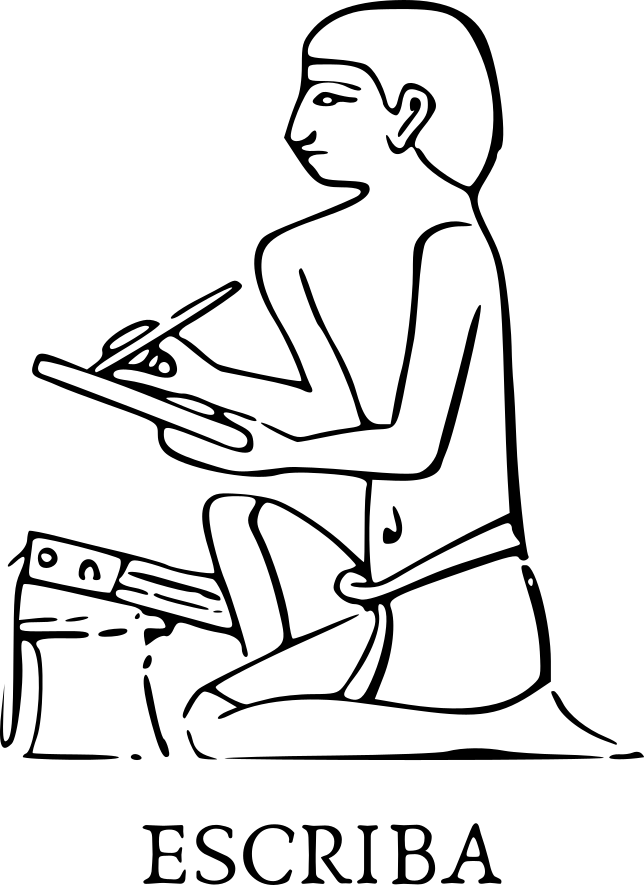
\includegraphics[scale=0.35]{static/logo.png}
    \end{figure}
    \vspace{1.5cm}

    % About
    \textsc{\large
      \textbf{An efficient and automated\\ \LaTeX \ project layout}
    }\\[0.25cm]

  \end{center}
\end{titlepage}

\blankpage
\chapter*{Abstract}

This is the official \ESCRIBA user guide. The tool allows for efficiently manage
large \LaTeX based projects and automate several tasks such us cleaning of the
working directory, code reformatting, linking of externally generated figures
and bibliography compilation.

In this manual, all required information for downloading, installing, creating a
new project and customizing it is presented.

The tool is still under heavy maintenance, so if you experience any issue or bug
while working with it, please open a new issue in the official board:
\href{https://github.com/jorgepiloto/escriba/issues}{https://github.com/jorgepiloto/escriba/issues}.

\vspace{4cm}
\textbf{Keywords:} \LaTeX, automated template, project documentation, academical
work

\blankpage

% Start the table of contents, figures and tables %
\maketableofcontents

% ---------- BEGIN OF CONTENT FILES -------------
\pagenumbering{arabic}
\chapter{The ESCRIBA project}

\ESCRIBA is just an efficient and automated \LaTeX project layout:

\begin{itemize}
  \item A project layout because it provides you with several directories
        for building documents making use of \LaTeX.
  \item It is automated, as it ships with a Makefile for cleaning, formatting,
        compiling and rendering your work.
  \item And finally, it is efficient because it saves you time!
\end{itemize}

When working with large academical works, it might be difficult to manage large
quantities of data and information. The only thing writer should care about is
writing. This is the main goal of \ESCRIBA.

In addition, this tool does not require from Ethernet access, meaning that you
can fully work locally and keep track of the changes by using a version control
system (VCS) such is \href{https://git-scm.com/}{Git}.

Finally, \ESCRIBA is an open-source software, released under
\href{https://github.com/jorgepiloto/escriba/blob/main/LICENSE}{Apache 2.0
  LICENSE}. This means that users are allowed to improve and contribute to the
project or even create a new one! The source code is hosted in
\href{https://github.com/jorgepiloto/escriba}{https://github.com/jorgepiloto/escriba}.


% ----------- END OF CONTENT FILES -------------


% Cite the bibliography
\printbibliography

\end{document}
